\subsection{RAG}
Retrieval-Augmented Generation (RAG) is an architecture paradigm that bases the output of Large Language Models (LLMs) on knowledge retrieved externally and related to a specific domain. RAG uses dynamic queries in a curated knowledge base during inference instead of relying solely on parametric knowledge during pre-training; therefore, directly injecting relevant context into the model prompt. The approach addresses two major limitations of standalone LLMs, namely knowledge staleness, which refers to a failure to access information obtained after training, and hallucination, i.e., a tendency to make statements that are plausible but not necessarily true in the absence of contextual support. As a result, RAG is recognized as a fundamental pattern in the enterprise artificial intelligence, being a basis of question-answering systems, document retrieval, customer support robots, and intelligent agents.

\subsubsection{Architecture}
\begin{figure}[H]
    \centering
    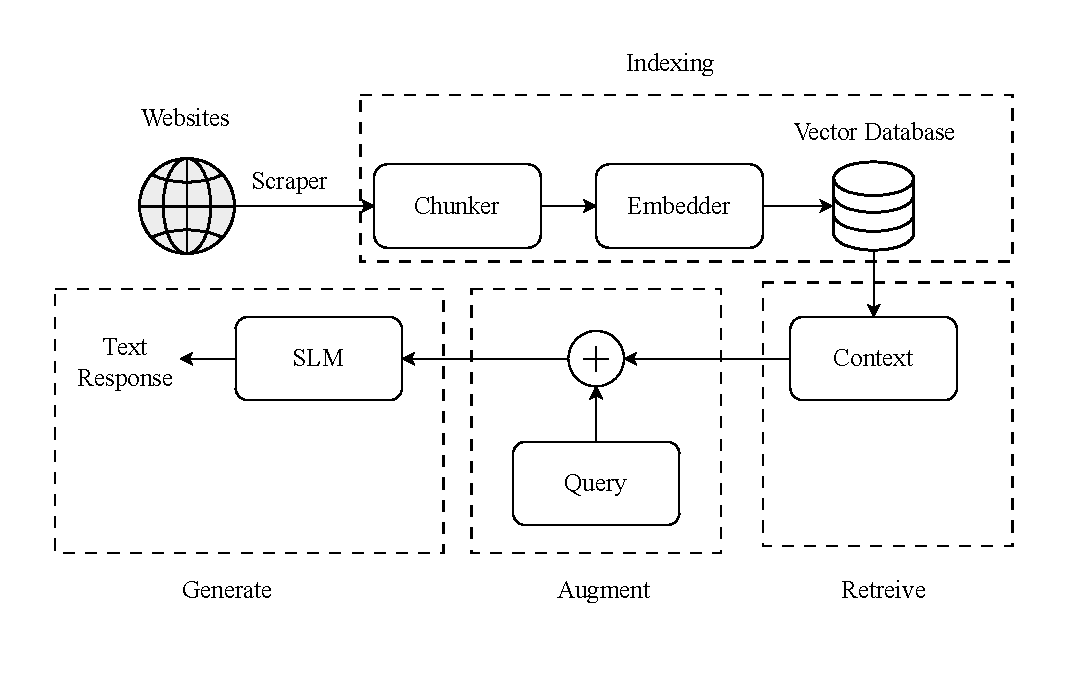
\includegraphics[width=\linewidth]{Images/RAG/Methodology/ASR-RAG.drawio.pdf}
    \caption{Architecture Of RAG}
\end{figure}

\subsubsection{Indexing Pipeline}
The indexing pipeline is committed with the task of transforming raw source documents into a format that can be effectively searched in semantic fashion at query time. This is a pre-processing step taken offline before any query of a user is serviced.

\textbf{Document Ingestion}

RAG systems support heterogeneous inputs. Typical sources include:
\begin{itemize}
    \item Structured data CSV files, database exports, spreadsheets.
    \item Unstructured documents PDFs, word documents, plain-text documents.
    \item Web content: URLs, scraped Web page data, scraped web data.
\end{itemize}

These inputs are normalised into a homogeneous text representation by an abstraction layer that loads documents, and their formatting and metadata are removed as needed, to pass on to the next stages.

\textbf{Chunking}

Raw documents are divided into smaller and semantically coherent units known as chunks. Chunking is an important design choice since embedding models have fixed context windows and accuracy of retrieval is dependent upon chunk granularity. The common strategies of applying chunking include:
\begin{itemize}
    \item \textbf{Fixed-size chunking:} Text is divided in terms of the number of tokens or characters, with or without overlap.
    \item \textbf{Sentence-level chunking:} Finding a linguistic coherence to sentence boundaries.
    \item \textbf{Semantic chunking:} Embedding distance text division by topic.
    \item \textbf{Recursive character splitting:} Hierarchically subdivision of paragraphs, sentences and words.
\end{itemize}

Chunk size and overlap are hyperparameters, which need to be adjusted to each application. Given a document of $N$ tokens, chunk size $c$, and overlap $o$, the number of chunks is:

\begin{equation}
    n_{\text{chunks}} = \left\lceil \frac{N - o}{c - o} \right\rceil
\end{equation}

Smaller chunks are less contextually complete and more precise in retrieval, whereas larger chunks have more of the context at the cost of relevance scores.

\textbf{Embedding Generation}

An embedding model learns each chunk and projects the textual data into a dense high-dimensional vector in a continuous semantic space. Semantic similarity is converted to geometrical proximity, which permits proximity-based retrieval. For a chunk $d_i$, its embedding vector is:

\begin{equation}
    \mathbf{v}_i = \text{Embed}(d_i) \in \mathbb{R}^{k}
\end{equation}

Embedding vectors are typically of dimensionality 768 to 3072, depending on what representational fidelity is required and storage overhead. To maintain the compatibility of the query encoding models, all the chunks should be embedded by the identical model that will encode the query at the retrieval stage.

\textbf{Vector Database Storage}

The resulting embeddings with their corresponding piece of text and their metadata are stored in a vector database. It is an approximate nearest-neighbour (ANN) optimised database that can allow sub-second time to perform similarity queries among millions of vectors. Vectors are paired with metadata, including source URL and document type, and a timestamp, to be used to do hybrid filtering of semantic similarity and structured attributes filters.

\subsubsection{Retrieval}

The online, real time aspect of the RAG pipeline is the retrieval stage. On the arrival of a user query, the system has to retrieve the most relevant document fragments in the vector database to provide context that can be used in the generation.

\textbf{Query Embedding}

The very model and configuration that are used in the indexing are used in the process of embedding the incoming user query:

\begin{equation}
    \mathbf{q} = \text{Embed}(q) \in \mathbb{R}^{k}
\end{equation}

The resulting query vector is placed on the same semantic space as the stored document chunk vectors, thus making similarity comparisons a meaningful process.

\textbf{Similarity Search}

A distance measure is used to compare the query vector with all the document vectors. The $k$ most similar chunks are fetched and delivered back as the context set. The similarity metrics used include:
\begin{itemize}
    \item \textbf{Cosine similarity} — this is an angle measure of the vectors and is resistant to magnitude differences:
    \begin{equation}
        \text{sim}_{\cos}(\mathbf{q},\, \mathbf{v}_i) = \frac{\mathbf{q} \cdot \mathbf{v}_i}{\|\mathbf{q}\|\,\|\mathbf{v}_i\|}
    \end{equation}

    \item \textbf{Dot product} — makes it easier to compute faster; it works well with normalised vectors:
    \begin{equation}
        \text{sim}_{\text{dot}}(\mathbf{q},\, \mathbf{v}_i) = \mathbf{q} \cdot \mathbf{v}_i
    \end{equation}

    \item \textbf{Euclidean distance (L2)} — the absolute spatial distance of vectors:
    \begin{equation}
        d_{L2}(\mathbf{q},\, \mathbf{v}_i) = \|\mathbf{q} - \mathbf{v}_i\|_2 = \sqrt{\sum_{j=1}^{k}(q_j - v_{ij})^2}
    \end{equation}
\end{itemize}

ANN algorithms used in most production vector-databases include HNSW (Hierarchical Navigable Small World) or IVF (Inverted File Index) to achieve scale retrieval without brute force search.

\subsubsection{Augmentation}

The augmentation stage builds the last prompt to be provided to the LLM. It combines the original query by the user with the retrieved bits of context in a form of a structured strict instruction-following format.

\textbf{Prompt Construction}

An effective RAG prompt usually has three elements:
\begin{itemize}
    \item \textbf{System instruction} — determines the role of the LLM and limits it to responding based on the context it is given.
    \item \textbf{Context block} — the textual concatenation of the $k$ best pieces of documents retrieved, explicitly marked.
    \item \textbf{User query} — the initial query or task posted by the user.
\end{itemize}

Time structure has a major impact on the quality of response. Context normally comes at the beginning before query to prime the attention of the model. XML tags or triple backticks mark the context and instructions to prevent prompt-injection threats.

\textbf{Context Management}

LLMs have set context windows (e.g.\ 8K, 32K, 128K tokens). The token budget available for retrieved context is:

\begin{equation}
    T_{\text{context}} = T_{\max} - T_{\text{system}} - T_{\text{query}}
\end{equation}

The augmentation layer needs to take care of context budgets:
\begin{itemize}
    \item \textbf{Truncation} — truncating the number of retrieved chunks or the length of the individual chunk.
    \item \textbf{Compression} — the summation of retrieved chunks before injection by a smaller LLM.
    \item \textbf{Selective inclusion} — score and filter chunks with relevance score less than relevance threshold and then include them.
\end{itemize}

\subsubsection{Generation}

The generation phase requests the augmented prompt to the LLM and provides the user with the response of the model. The LLM combines the context retrieved with the knowledge it has (in parametric form) to generate a grounded response.

\subsubsection{Evaluation Metrics}

\textbf{Faithfulness}

Measures the factual basis of the answer produced based on the context retrieved; i.e., the model does not produce hallucinatory claims that are not supported by the context. Given a generated answer with $n$ total statements and $n_{\text{supported}}$ statements grounded in the retrieved context:

\begin{equation}
    \text{Faithfulness} = \frac{n_{\text{supported}}}{n}
\end{equation}

\textbf{Answer and Context Relevance}
\begin{itemize}
    \item \textbf{Answer relevance} — determines how close the answer is to the initial query of the user, no matter whether it is factually correct or incorrect:
    \begin{equation}
        \text{AnswerRelevance}(A,\, q) = \frac{1}{m} \sum_{i=1}^{m} \text{sim}_{\cos}\!\left(\mathbf{q},\, \hat{\mathbf{q}}_i\right)
    \end{equation}

    \item \textbf{Context relevance} — measures the ratio of the retrieved context that is relevant to the query and thus over-retrieval and noise are identified:
    \begin{equation}
        \text{ContextRelevance}(\mathcal{C},\, q) = \frac{|\mathcal{C}_{\text{relevant}}|}{|\mathcal{C}|}
    \end{equation}
\end{itemize}

\textbf{Latency}

The end-to-end time, including embedding, vector search, prompt construction, and LLM inference:

\begin{equation}
    T_{\text{total}} = T_{\text{embed}} + T_{\text{search}} + T_{\text{prompt}} + T_{\text{LLM}}
\end{equation}

\textbf{Average Answer Length}

A base signal; extremely short responses can be signs of refusals or context loss, whereas extremely long responses can be signs of prompt or chunking difficulties:

\begin{equation}
    \bar{L} = \frac{1}{|\mathcal{Q}|} \sum_{i=1}^{|\mathcal{Q}|} \text{len}(A_i)
\end{equation}

\textbf{Answer Rate}

The accuracy of the system in responding to a query with a meaningful response, as opposed to rejecting the query on the basis of being under-contextualized:

\begin{equation}
    \text{AnswerRate} = \frac{|\{q \in \mathcal{Q} : A_q \neq \emptyset\}|}{|\mathcal{Q}|}
\end{equation}
